\documentclass[11pt]{article}

\usepackage{a4wide}
\usepackage[utf8]{inputenc}
\usepackage[russian]{babel}
\usepackage{graphicx}
\usepackage{amsmath}
\usepackage{amsthm}
\usepackage{amssymb}
\usepackage{amsfonts}

\newtheorem{theorem}{Теорема}
\newtheorem{defenition}{Определение}
\newtheorem{proposition}{Утверждение}

\newcommand*{\hm}[1]{#1\nobreak\discretionary{}{\hbox{$\mathsurround=0pt #1$}}{}}
\newcommand\abs[1]{\left\lvert#1\right\rvert}
\newcommand{\scalar}[2]{\left<#1,#2\right>}
\newcommand{\norm}[1]{\left\lVert #1 \right\lVert}
\renewcommand{\d}[1]{\ensuremath{\operatorname{d}\!{#1}}}
\newcommand{\const}{\ensuremath{\operatorname{const}}}
\newcommand{\sgn}{\ensuremath{\operatorname{sgn}}}

\begin{document}
\section{Задача 1}
\subsection{Формулировка}
Пусть имеется квадрат со стороной 1. Из каждой вершины квадрата внутрь проведены дуги окружностей с радиусом 1. Они окраничили внутри квадрата некоторую криволинейную фигуру. Необходимо найти её площадь.

%\includegraphics[scale=0.8]{pics/problem1_picture1.eps}

\subsection{Решение 1}
Назовём точки следующим образом:
%\includegraphics[scale=0.8]{pics/problem1_picture3.eps}
\begin{pspicture*}(0,0)(15,8.1807)
\psset{xunit=2.25551}
\psset{yunit=2.25551}
\newrgbcolor{000000}{0 0 0}
\newrgbcolor{ffffde}{1 1 0.870588}
\newrgbcolor{c5c2c5}{0.772549 0.760784 0.772549}
\newrgbcolor{a0a0a4}{0.627451 0.627451 0.643137}
\newrgbcolor{c0c0c0}{0.752941 0.752941 0.752941}
\psdots[linecolor=000000,dotscale=1,dotstyle=*,fillstyle=solid,fillcolor=000000](1.82985,0.381788)
\rput[tl](3.21374,0.783073)
{
u
}
\rput[tl](3.99317,1.02167)
{
w
}
\psarc[linecolor=000000,linewidth=0.01,linestyle=solid](1.82985,3.38179){6.76653}{-90}{0}
\psarc[linecolor=000000,linewidth=0.01,linestyle=solid](4.82985,3.38179){6.76653}{-180}{-90}
\psline[linecolor=000000,linewidth=0.01,linestyle=solid](4.82985,0.381788)(4.82985,3.38179)
\psline[linecolor=000000,linewidth=0.01,linestyle=solid](3.32985,2.97986)(4.82985,0.381788)
\psline[linecolor=000000,linewidth=0.01,linestyle=solid](4.82985,3.38179)(1.82985,3.38179)
\psarc[linecolor=000000,linewidth=0.01,linestyle=solid](4.82985,0.381788){6.76653}{90}{180}
\psarc[linecolor=000000,linewidth=0.01,linestyle=solid](1.82985,0.381788){6.76653}{-2.12037e-14}{90}
\rput[tl](2.05255,1.5466)
{
z
}
\rput[tl](4.82033,3.35997)
{
B
}
\psline[linecolor=000000,linewidth=0.01,linestyle=solid](1.82985,0.381788)(4.82985,0.381788)
\rput[tl](2.38659,2.13515)
{
y
}
\rput[tl](4.0568,2.11924)
{
y
}
\psline[linecolor=000000,linewidth=0.01,linestyle=solid](1.82985,3.38179)(1.82985,0.381788)
\psdots[linecolor=000000,dotscale=1,dotstyle=*,fillstyle=solid,fillcolor=000000](1.82985,3.38179)
\rput[tl](3.341,2.9464)
{
E
}
\psdots[linecolor=000000,dotscale=1,dotstyle=*,fillstyle=solid,fillcolor=000000](3.32985,2.97986)
\psline[linecolor=000000,linewidth=0.01,linestyle=solid](1.82985,0.381788)(3.32985,2.97986)
\psdots[linecolor=000000,dotscale=1,dotstyle=*,fillstyle=solid,fillcolor=000000](4.82985,3.38179)
\rput[tl](3.22965,1.73748)
{
x
}
\rput[tl](1.86167,0.369497)
{
D
}
\psdots[linecolor=000000,dotscale=1,dotstyle=*,fillstyle=solid,fillcolor=000000](4.82985,0.381788)
\rput[tl](4.37494,1.5466)
{
z
}
\rput[tl](2.35478,1.05349)
{
w
}
\rput[tl](4.88395,0.40131)
{
C
}
\rput[tl](1.81395,3.35997)
{
A
}
\end{pspicture*}

\end{document}